{\centering
  \small
  \textbf{This chapter is based on the following publication}
  \begin{quote}
    {Julien Tissier, Christophe Gravier, and Amaury Habrard. ``Near-lossless
    binarization of word embeddings''. In \textit{Proceedings of the AAAI
    Conference on Artificial Intelligence (AAAI 2019)}, volume 33, pages
    7104–7111, 2019.}
  \end{quote}
  \noindent\rule{\textwidth}{1pt}
}

\section{Introduction}
  \label{ch06:sec:introduction}
  Word embeddings are usually computed for a large vocabulary size and with
  vectors of many dimensions. In the literature, it is common to see a
  vocabulary of millions of words and vectors of hundreds of dimensions. With
  such characteristics, storing word embeddings require several gigabytes of
  memory space. For example, with a vocabulary of 2 million words and
  300-dimensional vectors, storing word embeddings require 2.4 gigabytes of
  memory space with real values encoded as \texttt{float}\footnote{A
  \texttt{float} commonly requires $32$ bits (= $4$ bytes) in memory.}. While
  learning and running models with word embeddings is not a problem for large
  computing servers, it becomes a concern to store word embeddings and run
  models which use them on embedded devices such as cell phones. Due to their
  limited memory and low computing power for floating-point arithmetic, it is
  hardly feasible in practice to do so. To overcome the problem of not being
  able to store word embeddings on memory-limited devices, NLP applications
  running on those devices usually send the data to process to large computing
  servers. The servers, which are able to store word embeddings and run the
  downstream model used for the task, handle the computations and return the
  results to the devices. This raises two concerns: (i) devices need an online
  connection to send data to computing servers; (ii) the privacy of device
  users is not preserved as their data are sent to computing servers and
  possibly stored server-side for other purposes. Reducing the size of word
  embeddings so downstream models could run on mobile devices would solve these
  two concerns as the computations would be done locally on the devices without
  needing to send data to a server, and therefore would allow one to run
  applications offline. \autoref{chap:methods-reduction} presented different
  methods to reduce the size of vector represensations like word embeddings.
  \medskip

  Making word embeddings consuming less space in memory is not the only
  condition to be able to run models on low-resource devices. Indeed, such
  devices are not efficient for floating-point computations, which prevents fast
  operations between real-valued vectors. To overcome this problem, a solution
  is to use binary operations. One can either \textit{binarize} the learning
  parameters of the model~\citep{hubara2016binarized} or \textit{binarize}
  vector representations (see~\autoref{ch04:sec:integer-vectors}
  in~\autoref{chap:methods-reduction} for a review of such methods). The
  contribution described in this chapter stands in the second category. As
  explained in~\autoref{ch04:sec:integer-vectors}
  of~\autoref{chap:methods-reduction}, vector operations are much faster with
  binary representations as they can be computed with bitwise operators instead
  of floating-point arithmetic. However, binary representations need to be
  aligned with CPU registers to fully take advantage of fast binary operations,
  which imposes the binary vectors to have a length of 64, 128 or 256 bits.
  Nevertheless, mapping words to binary codes is not enough as the vectors are
  then used in NLP applications. They also need to encode semantic and syntactic
  information; the objective then becomes to find binary vectors which preserve
  the linguistic properties and are small enough to fit in CPU registers. Note
  here that there is a difference between learning binary word embeddings from
  scratch (\textit{i.e.} directly from text corpora or from external linguistic
  resources) and transforming pre-trained real-valued word embeddings. Most
  common models used to learn word embeddings propose to download pre-trained
  word vectors~\citep{mikolov2013distributed, pennington2014glove,
  bojanowski2016enriching, tissier2017dict2vec}, each one with its own specific
  encoded linguistic information due to its learning scheme. Finding a method
  which can binarize pre-trained word embeddings is more useful than learning
  binary vectors from scratch because they would direcly encode the specific
  linguistic information of the original pre-trained word vectors instead of
  having to re-train the binary vectors with the appropriate learning
  scheme.\medskip

  This chapter presents the second contribution of this thesis: a novel model to
  solve the problem of producing binary word vectors from pre-trained
  real-valued embeddings while preserving their linguistic and semantic
  information so they can be used in downstream models, requiring less memory
  space and speeding up vector operations. This model is based on an autoencoder
  architecture. The main results of this contribution are:

  \begin{itemize}
    \item The model architecture can transform any real-valued vectors to
      binary vectors of any size (\textit{e.g.} 64, 128 or 256 bits to be in
      adequacy with CPU register sizes).
    \item The architecture has the ability to reconstruct original real-valued
      word vectors from the binary ones with high accuracy.
    \item Binary vectors \textbf{use 97\% less memory space} than the original
      real-valued vectors with only a loss of $\sim$2\% in accuracy on word
      semantic similarity, text classification and sentiment analysis tasks.
    \item A top-K query is \textbf{30 times faster} with binary vectors than
      with real-valued vectors.
  \end{itemize}

  \noindent This model is named \texttt{NLB} for
  ``\textbf{N}ear-\textbf{L}ossless \textbf{B}inarization of word embeddings''
  in the rest of this chapter. In the following,
  \autoref{ch06:sec:nlb-autoencoder} describes the autoencoder architecture used
  to \textit{binarize} real-valued word embeddings into binary vectors while
  \autoref{ch06:sec:experiments} presents the training settings and the
  evaluation protocol. Finally,~\autoref{ch06:sec:nlb-results} analyzes the
  performances of binary vectors on different downstream NLP task, as well as
  their semantic properties and their influence on the speed of vector
  operations. Entire source code to generate and evaluate binary vectors is
  publicly available
  online\footnote{\url{https://github.com/tca19/near-lossless-binarization}}.

\section{Binarizing word vectors with an autoencoder}
  \label{ch06:sec:nlb-autoencoder}
  As explained in the introduction of this chapter, transforming real-valued
  embeddings to binary vectors has the dual benefit of reducing the memory space
  of word embeddings and making vector operations faster. A naive approach to
  produce binary vectors is to map each value $\mathbf{x}_{[i]}$ of a
  pre-trained real-valued word vector $\mathbf{x}$ to $0$ if $\mathbf{x}_{[i]} <
  0$ and to $1$ otherwise. This method does not require any training but suffers
  from an important drawback: binary vectors \emph{have the same number of
  dimensions} as the original ones. Available pre-trained word embeddings
  typically have lengths of $100$, $200$ or $300$ dimensions so to produce
  binary vectors of $64$, $128$ or $256$ bits (to be aligned with CPU registers
  size), one has to train from scratch real-valued embeddings with those
  dimensions and then apply the naive binarization. Results
  in~\autoref{ch06:subsec:performances-naive} show that it is slower and less
  efficient than the proposed method which directly transforms vectors with the
  appropriate binary size.

  \subsection{Autoencoder architecture}
    Let $\mathcal{V}$ be a vocabulary of words and $\mathbf{M} \in
    \mathbb{R}^{|\mathcal{V}| \times d}$ the embedding matrix whose rows are
    $d$-dimensional real-valued vectors representing the embedding of each word
    of $\mathcal{V}$. The main objective is to transform each word vector
    $\mathbf{x}_i$ (\textit{i.e} each row of the matrix $\mathbf{M}$) into a
    binary vector $\mathbf{b}_i$ of $n$ dimensions with $n \ll (d \times k)$
    where $k$ corresponds to the encoding size of real-valued numbers in memory
    (\textit{e.g.} 32 bits for standard single-precision floating-point numbers)
    while preserving the semantic information contained in $\mathbf{x}_i$. The
    proposed method achieves this objective by using an autoencoder model
    composed of two parts: an encoder which binarizes a word vector $\mathbf{x}$
    to $\Phi(\mathbf{x})$ and a decoder which reconstructs a real-valued vector
    $\hat{\mathbf{y}}$ from $\Phi(\mathbf{x})$. The binarized vector is
    therefore the latent representation $\Phi(\mathbf{x})$ of the
    autoencoder.~\autoref{ch06:img:nlb-autoencoder} summarizes this model
    architecture.

    \begin{figure}[h]
      \begin{center}
        \centerline{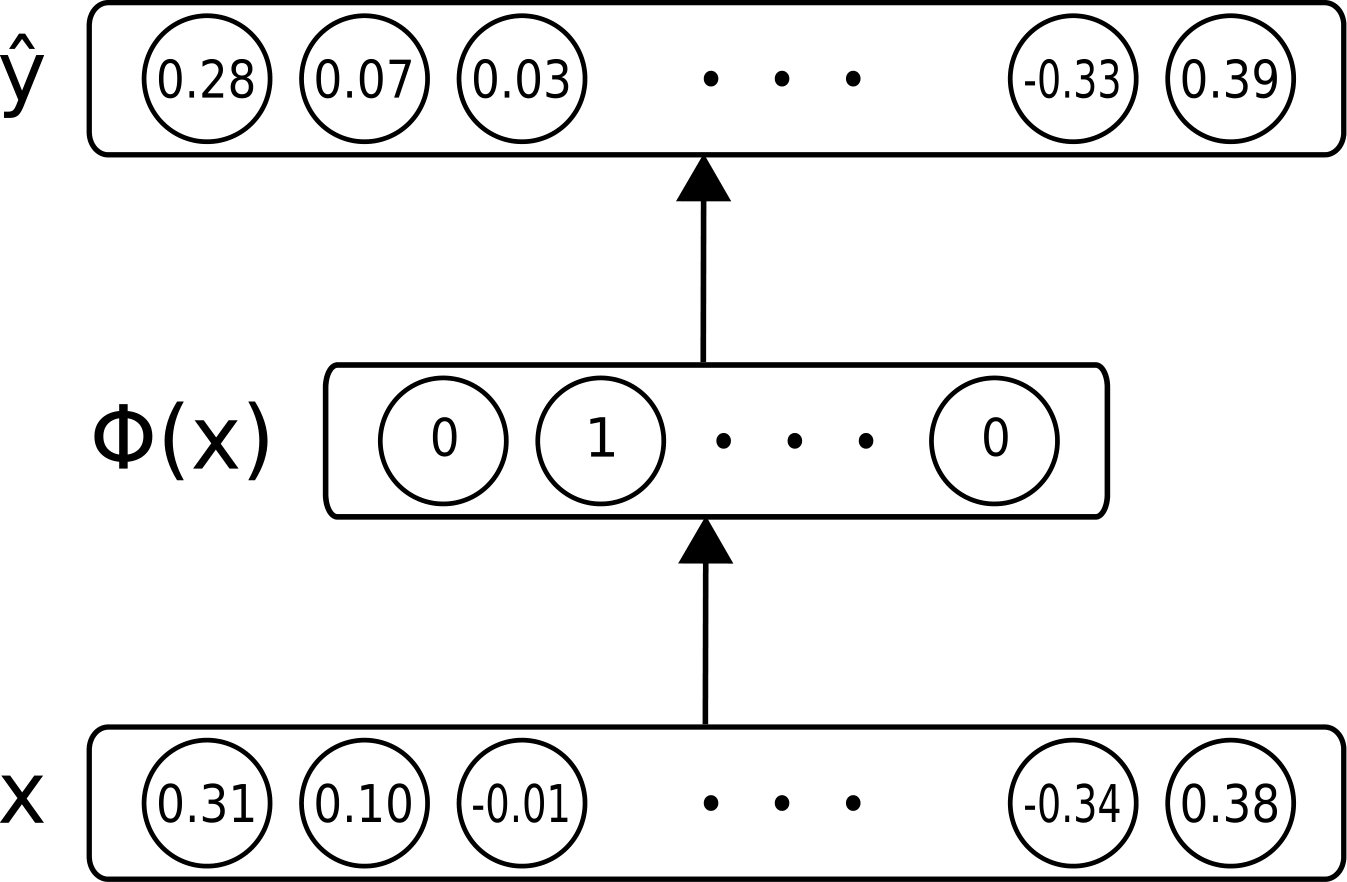
\includegraphics[width=0.6\linewidth]{ch06-binary-autoencoder}}
        \caption[Autoencoder architecture used to binarize word vectors.]
        {Autoencoder architecture used to binarize word vectors and reconstruct
        a real-valued representation. The model can learn $\Phi(\mathbf{x})$
        vectors of any arbitrary size. To be aligned with CPU registers, the
        length of $\Phi(\mathbf{x})$ is suggested to be 64, 128 or 256 bits.}
        \label{ch06:img:nlb-autoencoder}
      \end{center}
    \end{figure}

    \subsubsection{Encoding to binary vectors}
      Let $\mathbf{W} \in \mathbb{R}^{n \times d}$ be a $n \times d$ matrix and
      $\mathbf{x}_i \in \mathbb{R}^d$ a $d$-dimensional word embedding. The
      binarized vector $\mathbf{b}_i$ of $\mathbf{x}_i$ is defined as:

      \begin{equation}
        \mathbf{b}_i = \Phi(\mathbf{x}_i)
                     = h(\mathbf{W} \cdot \mathbf{x}_i{}^\top)
      \end{equation}
      where $h(.)$ is an element-wise function which outputs a bit given a real
      value, such as the Heaviside step function. The dimension of $\mathbf{W}$
      is $(n \times d)$ \textit{i.e.} the desired size $n$ of binary vectors and
      the size $d$ of the original real-valued vector $\mathbf{x}_i$. Therefore
      this model can be used to generate binary vectors of any size by choosing
      the appropriate value for $n$, independently of the size of the original
      real-valued vectors.

    \subsubsection{Reconstructing a real-valued vector}
      The latent representation $\Phi(\mathbf{x}_i)$ is then used to compute a
      reconstructed vector $\hat{\mathbf{y}}_i$ as:

      \begin{equation}
        \hat{\mathbf{y}}_i = f(\mathbf{W}{}^\top \cdot \Phi(\mathbf{x}_i)
                             + \mathbf{c})
      \end{equation}
      where $\mathbf{c}$ is a $d$-dimensional real-valued bias vector and $f$ is
      an element-wise non-linear function. The $f$ function must be chosen such
      that its output domain is the same as the range of values in the input
      real-valued embedding $\mathbf{x}_i$ of the autoencoder. Indeed, if for
      example input embeddings all have negative values and $f$ is a function
      whose output domain is $\mathbb{R}^{+}$, values of vectors
      $\hat{\mathbf{y}}_i$ would be positive. Since autoencoders are trained so
      their outputs are close to their inputs, it would not be possible to train
      it correctly in this case (inputs are negative, outputs would be
      positive).\medskip

      The proposed model is trained to be able to reconstruct word embeddings.
      Most of the existing pre-trained word embeddings have values which are
      within the $[-1, 1]$ range. Following the imposed condition on $f$, the
      hyperbolic tangent function is used as $f$ in the proposed model because
      its output domain is also the $[-1, 1]$ range. For the few word vectors
      having values outside this range, their values are clipped to be in $[-1,
      1]$ before being used as inputs in the autoencoder model. Our experiments
      showed that the clipping step does not alter the quality of the
      pre-trained vectors (word semantic similarity scores stay the same for
      \texttt{GloVe} vectors) as most of the vector values are already within
      this range.

  \subsection{Objective function}
    \label{ch06:subsec:objective-function}
    The reconstruction loss $\ell_{rec}$ for a vector $\mathbf{x}_i$ is defined
    as the mean squared error between this original vector $\mathbf{x}_i$ and
    the reconstructed output vector $\hat{\mathbf{y}}_i$ of the autoencoder:
    \begin{equation}
      \ell_{rec}(\mathbf{x}_i) = \frac{1}{d} \left\lVert
        \mathbf{x}_i - \hat{\mathbf{y}}_i \right\rVert^2
                               = \frac{1}{d} \sum_{j=1}^d
        (\mathbf{x}_{i_{[j]}} - \hat{\mathbf{y}}_{i_{[j]}})^2
    \end{equation}
    where $\mathbf{x}_{i_{[j]}}$ (resp. $\hat{\mathbf{y}}_{i_{[j]}}$) is the
    $j$-th value of the vector $\mathbf{x}_i$ (resp. $\hat{\mathbf{y}}_{i}$).
    The autoencoder is trained to minimize this loss for all word vectors
    $\mathbf{x}_i$ in the embedding matrix $\mathbf{M}$. Learning the optimal
    parameters $\mathbf{W}$ and $\mathbf{c}$ of the autoencoder by minimizing
    this loss function produces good reconstructed vectors but the latent binary
    representations of words learned by the model are not preserving the
    semantic properties of original real-valued vectors. Indeed, since the model
    is trained to only minimize the reconstruction loss, the learned matrix
    $\mathbf{W}$ used in the encoding step discards too much similarity
    information between related word vectors from the original vector space in
    favor of the reconstruction (this behavior has been observed in practice in
    the experiments). To solve this problem, a regularization term has been
    added into the objective function of the model, defined as:
    \begin{equation}
      \ell_{reg} = \frac{1}{2} \left\lVert \mathbf{W}{}^\top \mathbf{W}
                                            - \mathbf{I} \right\rVert^2
    \end{equation}
    This term aims to minimize the correlation between the dimensions of latent
    binary vectors. Since the model aims to produce small-sized binary
    embeddings which preserve linguistic information, it needs to encode as much
    linguistic information as possible across all the dimensions of binary
    vectors. Therefore, minimizing the correlation between the dimensions of
    binary vectors is crucial to avoid duplicate information. This
    regularization has the effect of preserving the information contained in the
    real-valued embeddings, so vectors that are close in the original vector
    space are also close in the binary vector space. The balance between the
    influence of the reconstruction loss and the regularization loss is achieved
    with the $\lambda_{reg}$ parameter. The global objective function
    $\mathcal{L}$ of the models is:
    \begin{equation}
      \mathcal{L} = \sum_{\mathbf{x}_i \in \mathbf{M}}
                    \ell_{rec}(\mathbf{x}_i) + \lambda_{reg} \; \ell_{reg}
    \end{equation}

    \medskip
    \textbf{Note here that the same parameter matrix $\mathbf{W}$ is used both
    for the encoder and for the decoder part in the \texttt{NLB} autoencoder
    model}. This is actually motivated by the fact that the function $h(\cdot)$
    involved during the encoding step to tranform real-valued vectors with
    $\Phi(\cdot)$ is non-differentiable so it is not possible to compute a
    gradient to update the parameters of the encoder with the gradient descent
    technique. It is assumed that:
    \begin{equation}
      \frac{\partial \Phi(\mathbf{x}_i)}{\partial \mathbf{W}} = 0
    \end{equation}
    However, the values of the $\mathbf{W}$ matrix used during the encoding step
    can still be updated thanks to the information provided by the decoder and
    its gradient, which is:
    \begin{equation}
      \frac
        {\partial \left\lVert \mathbf{x}_i - \hat{\mathbf{y}}_i \right\rVert^2}
        {\partial \mathbf{W}{}^\top}
    \end{equation}
    Since the matrices $\mathbf{W}$ and $\mathbf{W}{}^\top$ have the same values,
    the derivative of the global loss $\mathcal{L}$ with respect to
    $\mathbf{W}{}^\top$ is used to update the values of $\mathbf{W}$. The
    autoencoder is then trained with the stochastic gradient descent technique
    (SGD) to solve the optimization problem of minimizing the global loss.  The
    objective function of the \texttt{NLB} autoencoder model is both non-convex
    and non-smooth due to the non-differentiable function $h(\cdot)$. Despite
    the fact that proving a general convergence is a hard problem, it has been
    observed in practice that the regularization term plays an important role
    and allows the model to converge to a local optimum (without the
    regularization term, the model oscillates and the bits in  binary vectors
    keep flipping values at each iteration of the SGD optimization).

\section{Experimental setup}
  \label{ch06:sec:experiments}
  This section presents the settings and the hyperparameters used to train the
  \texttt{NLB} autoencoder model (\autoref{ch06:subsec:training-settings}). It
  also describes the evaluation protocol followed to measure the performances of
  the binary and reconstructed vectors on several tasks, which are commonly used
  to evaluate word representations
  (see~\autoref{ch01:sec:word-embeddings-evaluation}
  in~\autoref{chap:preliminaries}): intrinsic tasks with a word semantic
  similarity and a word analogy task
  (\autoref{ch06:subsec:protocol-intrinsic-tasks}); and extrinsic tasks with a
  document classification, a question classification and a sentiment analysis
  task (\autoref{ch06:subsec:protocol-extrinsic-tasks}). Another task (top-K
  queries) has been run to evaluate the computation efficiency of binary vectors
  (\autoref{ch06:subsec:protocol-speed-task}).

  \subsection{Training settings}
    \label{ch06:subsec:training-settings}
    \subsubsection{Pre-trained word embeddings}
      The \texttt{NLB} model produces binary vectors from pre-trained word
      embeddings. The model has been trained to binarize several different
      pre-trained word embeddings:

      \begin{itemize}
        \item \texttt{dict2vec}~\citep{tissier2017dict2vec} which contains 2.3M
          word vectors and has been trained on the full English Wikipedia
          corpus.
        \item \texttt{fasttext}~\citep{bojanowski2016enriching} which contains
          1M word vectors and has also been trained on the full English
          Wikipedia corpus.
        \item \texttt{GloVe}~\citep{pennington2014glove} which contains 400K
          word vectors and has been trained on the English Wikipedia and the
          Gigaword 5 corpora.
      \end{itemize}
      All word vectors have 300 dimensions. The learning hyperparameters used
      are the ones from their respective paper. Since the three word embeddings
      are based on different learning methods (derivation of the Skip-gram model
      for \texttt{dict2vec} and \texttt{fasttext}, matrix factorization for
      \texttt{GloVe}), this demonstrates that the \texttt{NLB} model is general
      and works for all kinds of pre-trained real-valued vectors, independently
      of the method used to learn them.

    \subsubsection{Hyperparameters of the \texttt{NLB} autoencoder model}
      The size $n$ of the latent representation of the autoencoder (which
      corresponds to the length of binary vectors) has been consecutively set to
      $64$, $128$, $256$ and $512$ to produce binary vectors with the same
      number of bits. The optimal other hyperparameters are found by using a
      grid search and are selected to minimize the reconstruction loss and the
      regularization loss described in \autoref{ch06:subsec:objective-function}.
      The model uses a batch size of $75$ real-valued vectors for the stochastic
      gradient descent, 10 training epochs for \texttt{dict2vec} and
      \texttt{fasttext} (\textit{i.e.} each vector of the embedding matrix
      $\mathbf{M}$ is seen 10 times) and 5 epochs for \texttt{GloVe} (the
      autoencoder converges faster due to the smaller number of word vectors in
      \texttt{GloVe}) and a learning rate of $0.001$. The regularization
      hyperparameter $\lambda_{reg}$ depends on the pre-trained vectors used and
      the binary vector size. It varies from $1$ to $4$ in the experiments but
      its influence on the performance is small ($\sim$2\% variation).
      %The training and performance benchmarks have been run on an Intel Xeon
      %1246 v3. Source code is written in C and compiled with GCC 7.3 and the
      %highest level of optimization available (\verb+-O3 -march=native+).

  \subsection{Intrinsic evaluation tasks}
    \label{ch06:subsec:protocol-intrinsic-tasks}
    \subsubsection{Word semantic similarity}
      Both binary and reconstructed vectors are evaluated with the standard
      method of the word semantic similarity task, explained in details
      in~\autoref{ch01:subsubsec:semantic-similarity}
      of~\autoref{chap:preliminaries}. This task consists in computing the
      Spearman's rank correlation coefficient between the similarity scores
      attributed by humans to pairs of words and the similarity scores computed
      with the vectors of the words. The similarity score for real-valued vectors
      is computed with their cosine similarity while the similarity score of
      two binary vectors ($\mathbf{b}_1, \mathbf{b}_2$) is computed with the
      Sokal \& Michener similarity function~\citep{sokal1958statistical} defined
      as:

      \begin{equation}
        \text{sim}(\mathbf{b}_1, \mathbf{b}_2) = {n_{11} + n_{00} \over {n}}
      \end{equation}
      where $n_{11}$ (resp. $n_{00}$) is the number of bits in $\mathbf{b}_1$
      and $\mathbf{b}_2$ that are both set to 1 (resp. 0) simultaneously and $n$
      is the size of binary vectors. The datasets used for this task are:
      \begin{itemize}
        \item MEN~\citep{bruni2014multimodal}
        \item RW~\citep{luong2013better}
        \item SimLex~\citep{hill2015simlex}
        \item SimVerb-3500~\citep{gerz2016simverb}
        \item WordSim-353~\citep{finkelstein2001placing}
      \end{itemize}

    \subsubsection{Word analogy}
      Binary and reconstructed vectors are also evaluated on the word analogy
      task, described in more details in~\autoref{ch01:subsubsec:word-analogy}
      of~\autoref{chap:preliminaries}. This evaluation follows the standard
      protocol used by~\citet{mikolov2013distributed}. The task consists in
      finding the word $d$ in questions like ``$a$ is to $b$ as $c$ is to $d$''
      given the words $a$, $b$ and $c$. First, the vector $\mathbf{v} =
      \mathbf{v}_b - \mathbf{v}_a + \mathbf{v}_c$ is computed with the
      respective word vectors of $a$, $b$ and $c$. Then, if the closest vector
      of $\mathbf{v}$ in the embedding matrix is the vector associated to the
      word $d$, the analogy is correct. The score on the task reports the
      fraction of correctly guessed analogies among all analogies. For binary
      vectors, the vector addition is replaced by the \texttt{OR} bitwise
      operator and the vector subtraction by the \texttt{AND NOT} operator
      because adding or subtracting bits does not really make sense in the
      binary vecor space (\textit{e.g.} subtracting the bit 1 to the bit 0). The
      closest vector of $\mathbf{v}$ is found by selecting the vector with the
      highest cosine (resp. Sokal \& Michener) similarity among all the
      real-valued (resp. binary) vectors of the embedding matrix $\mathbf{M}$.
      The evaluation dataset of word analogies is separated into two parts: one
      consists of analogies about countries and currencies (semantic analogies),
      the other one about English grammar (syntactic analogies), as done
      in~\citep{mikolov2013distributed}.

  \subsection{Extrinsic evaluation tasks}
    \label{ch06:subsec:protocol-extrinsic-tasks}
    The two intrinsic tasks measure how well the semantic and syntactic
    information from the original real-valued vectors has been preserved in the
    binary and reconstructed vectors, but they do not evaluate how well those
    vectors perform in downstream tasks. To evaluate the quality of binary and
    reconstructed vectors when they are used in downstream models, several
    additional evaluations have been performed on:
    \begin{itemize}
      \item document classification;
      \item question classification;
      \item sentiment analysis.
    \end{itemize}
    A detailed description of those tasks has been presented
    in~\autoref{ch01:subsec:extrinsic-evaluation}
    of~\autoref{chap:preliminaries}. The evaluation follows the same protocol as
    described in the literature~\citep{zhang2015character, joulin2016bag} which
    consists in predicting the correct label given the Bag-of-Words
    representation of a text. A single hidden layer neural network where the
    input weights have been initialized with the binary or reconstructed vectors
    is used. The input weights are freezed during training so that the
    classification accuracy solely depends on the vectors used to initialize the
    neural network weights. The datasets used for the three tasks are:
    \begin{itemize}
      \item AG-News and DBpedia for the document classification task;
      \item Yahoo Answers for the question classification;
      \item Amazon and Yelp reviews (both polarity and full) for the sentiment
        analysis task.
    \end{itemize}
    Each dataset is split into a training and a test file and the same training
    and test files are used for all the models evaluating the binary and
    reconstructed vectors. Accuracy results are
    reported in~\autoref{ch06:tab:results-binary-classification} for binary
    vectors and in~\autoref{ch06:tab:results-reconstructed-classification} for
    reconstructed vectors.

  \subsection{Computation speed evaluation}
    \label{ch06:subsec:protocol-speed-task}
    Evaluation tasks presented in~\autoref{ch06:subsec:protocol-intrinsic-tasks}
    or in~\autoref{ch06:subsec:protocol-extrinsic-tasks} only evaluate the
    quality of binary word embeddings from a linguistic point of view, based on
    their encoded information or on how useful the binary vectors are when they
    are used in downstream models. However, as explained
    in~\autoref{ch06:sec:introduction} of this chapter or
    in~\autoref{chap:methods-reduction}, binary vectors have the advantage of
    speeding up vector operations because they can be done with bitwise
    operators. To measure how much faster the computations are, a top-K queries
    evaluation is performed. It consists in finding the \textit{K} closest
    vectors given a single word vector query. The closest vectors are the ones
    with the highest similarity to the query vector (Sokal \& Michener
    similarity for binary vectors, cosine similarity for real-valued ones) and
    are found by performing a linear scan across all vectors. Two execution
    times are measured for both binary and real-valued vectors: the time it
    takes to get the results once the vectors are loaded in memory and the time
    it takes to load the vectors and perform the query.\medskip

\section{Results and binary vectors analysis}
  \label{ch06:sec:nlb-results}
  This section presents the performances of binary and reconstructed vectors
  produced by the \texttt{NLB} autoencoder model on different evaluation tasks,
  respectively in~\autoref{ch06:subsec:performances-binary} and in
  \autoref{ch06:subsec:performances-reconstructed}. The computational speed
  benefits of binary vectors are detailed in
  \autoref{ch06:subsec:performances-speed}. Comparisons with other binarization
  methods are made in~\autoref{ch06:subsec:performances-naive} and
  in~\autoref{ch06:subsec:performances-others}.
  Lastly,~\autoref{ch06:subsec:qualitative-analysis} carries out an analysis of
  the semantic properties encoded into binary vectors.

  \subsection{Binary word embeddings performances}
    \label{ch06:subsec:performances-binary}
    \subsubsection{Word semantic similarity}
      \autoref{ch06:tab:results-binary-semantic} reports the Spearman's rank
      correlation scores obtained by the binarized vectors learned by the
      \texttt{NLB} autoencoder model (\texttt{NLB} row) and the scores of the
      original real-valued vectors ($\mathbb{R}$ column) whose size is 9,600
      bits per vector (300 dimensions, 32 bits per \texttt{float} value) for
      different pre-trained word embeddings (\texttt{dict2vec},
      \texttt{fasttext} and \texttt{GloVe}). The best scores of binarized
      vectors are reached with 256 or 512 bits. For \texttt{fasttext} and
      \texttt{GloVe}, the results of binary vectors are very close to the scores
      obtained by the original real-valued vectors (average absolute difference
      is smaller than $0.01$). For \texttt{dict2vec}, the deviation is larger
      (between $0.03$ and $0.05$) but still in the same order of magnitude.
      Binarizing word vectors can lead to better scores compared to the original
      ones ($\mathbb{R}$ column), for example the 512-bit binary vectors of
      \texttt{fasttext} on WordSim ($0.703$ against $0.697$) or the 256-bit binary
      vectors of \texttt{GloVe} on SimVerb ($0.229$ against $0.227$). Moreover,
      the 64-bit binary vectors of \texttt{dict2vec} are better than the
      real-valued \texttt{GloVe} embeddings (which uses 9,600 bits of
      information per vector so binary codes are 150 times smaller) on SimVerb
      ($0.253$ against $0.227$) and WordSim ($0.637$ against $0.609$). This
      demonstrates that the method can produce rich semantically-related small
      binary codes but also more generally, that \textit{binary vectors can
      encode the same semantic information as real-valued vectors}.\bigskip

      % Table with scores of binary vectors on word semantic similarity task.
      \begin{table}[b!]
        \centering
        \resizebox{\linewidth}{!}{
          \begin{tabular}{@{}lcccccrcccccrccccc@{}}
          \toprule[0.15em]
            & \multicolumn{5}{c}{\texttt{dict2vec}} & \phantom{}
            & \multicolumn{5}{c}{\texttt{fasttext}} & \phantom{}
            & \multicolumn{5}{c}{\texttt{GloVe}}\\

            \cmidrule(lr){2-6} \cmidrule(lr){8-12} \cmidrule(lr){14-18}
            & $\mathbb{R}$ & 64 & 128 & 256 & 512 &
            & $\mathbb{R}$ & 64 & 128 & 256 & 512 &
            & $\mathbb{R}$ & 64 & 128 & 256 & 512 \\
            \midrule
              % raw  64     128         256       512
            MEN & 0.746 &&&&&& 0.807 &&&&&& 0.737\\
              \multicolumn{1}{c}{\texttt{NLB}}
                &-& 0.661 & \textbf{0.713} & 0.703 & 0.713 &
                &-& 0.579 & 0.720 & 0.759 & \textbf{0.763} &
                &-& 0.461 & 0.633 & 0.694 & \textbf{0.727}\\
              \multicolumn{1}{c}{\texttt{LSH}}
                &-& 0.477 & 0.562 & 0.626 & 0.678 &
                &-& 0.477 & 0.607 & 0.700 & 0.750 &
                &-& 0.508 & 0.620 & 0.649 & 0.710\\\\

            RW & 0.505 &&&&&& 0.538 &&&&&& 0.412\\
              \multicolumn{1}{c}{\texttt{NLB}}
                &-& 0.365 & 0.420 & 0.456 & 0.456 &
                &-& 0.368 & 0.447 & \textbf{0.527} & 0.527 &
                &-& 0.251 & 0.343 & \textbf{0.407} & 0.402\\
              \multicolumn{1}{c}{\texttt{LSH}}
                &-& 0.264 & 0.372 & 0.417 & \textbf{0.462} &
                &-& 0.345 & 0.403 & 0.475 & 0.465 &
                &-& 0.263 & 0.330 & 0.358 & 0.383\\\\

            SimLex & 0.452 &&&&&& 0.441 &&&&&& 0.371\\
              \multicolumn{1}{c}{\texttt{NLB}}
                &-& 0.320 & 0.381 & \textbf{0.448} & 0.429 &
                &-& 0.251 & 0.380 & \textbf{0.446} & 0.430 &
                &-& 0.205 & 0.314 & \textbf{0.372} & 0.368\\
              \multicolumn{1}{c}{\texttt{LSH}}
                &-& 0.296 & 0.359 & 0.402 & 0.395 &
                &-& 0.287 & 0.320 & 0.386 & 0.411 &
                &-& 0.247 & 0.305 & 0.331 & 0.346\\\\

            SimVerb & 0.417 &&&&&& 0.356 &&&&&& 0.227\\
              \multicolumn{1}{c}{\texttt{NLB}}
                &-& 0.253 & 0.366 & \textbf{0.384} & 0.355 &
                &-& 0.192 & 0.267 & 0.337 & \textbf{0.351} &
                &-& 0.078 & 0.187 & 0.229 & \textbf{0.230}\\
              \multicolumn{1}{c}{\texttt{LSH}}
                &-& 0.220 & 0.275 & 0.316 & 0.369 &
                &-& 0.205 & 0.233 & 0.307 & 0.302 &
                &-& 0.146 & 0.174 & 0.188 & 0.207\\\\

            WordSim & 0.725 &&&&&& 0.697 &&&&&& 0.609\\
              \multicolumn{1}{c}{\texttt{NLB}}
                &-& 0.637 & \textbf{0.716} & 0.696 & 0.666 &
                &-& 0.503 & 0.691 & 0.700 & \textbf{0.703} &
                &-& 0.301 & 0.449 & 0.566 & \textbf{0.603}\\
              \multicolumn{1}{c}{\texttt{LSH}}
                &-& 0.455 & 0.569 & 0.649 & 0.655 &
                &-& 0.467 & 0.532 & 0.586 & 0.638 &
                &-& 0.411 & 0.444 & 0.505 & 0.578\\
          \bottomrule[0.15em]
        \end{tabular}}
        \caption[Evaluation of binary and real-valued vectors on a semantic
        similarity task.]{Semantic similarity scores on several datasets for
        binary vectors produced with the proposed method (\texttt{NLB} row) or
        produced with the Local Sensitive Hashing method (\texttt{LSH} row) with
        different vector sizes: 64, 128, 256 and 512 bits. Several pre-trained
        word embeddings have been binarized (\texttt{dict2vec},
        \texttt{fasttext} and \texttt{GloVe}). For each dataset, scores of
        original real-valued vectors are also reported ($\mathbb{R}$ column).}
        \label{ch06:tab:results-binary-semantic}
      \end{table}

      \noindent The average of word semantic similarity scores of all datasets
      (computed with the Fisher's transformation) for binary and original word
      embeddings (whose size is 9,600 bits per vector) are plotted
      in~\autoref{ch06:img:plot-binary-vectors}. The 512-bit binary vectors of
      \texttt{GloVe} are on par with the real-valued vectors. However the
      performance loss is greater for \texttt{fasttext} and \texttt{dict2vec}. A
      possible explanation is that those word embeddings contain more vectors to
      binarize (1M vectors for \texttt{fasttext} and 2.3M for
      \texttt{dict2vec} whereas \texttt{GloVe} only has 400K vectors). Since the
      binary vector space has a finite size depending on the binary vector size,
      it becomes harder for the autoencoder to find a distribution of the binary
      vectors which preserves the semantic similarity between vectors when the
      number of vectors is larger.

      \begin{figure}[b!]
        \centering
        % if the size is larger than 0.75 \linewidth, it completely fucks up the
        % formatting of the rest of the chapter
        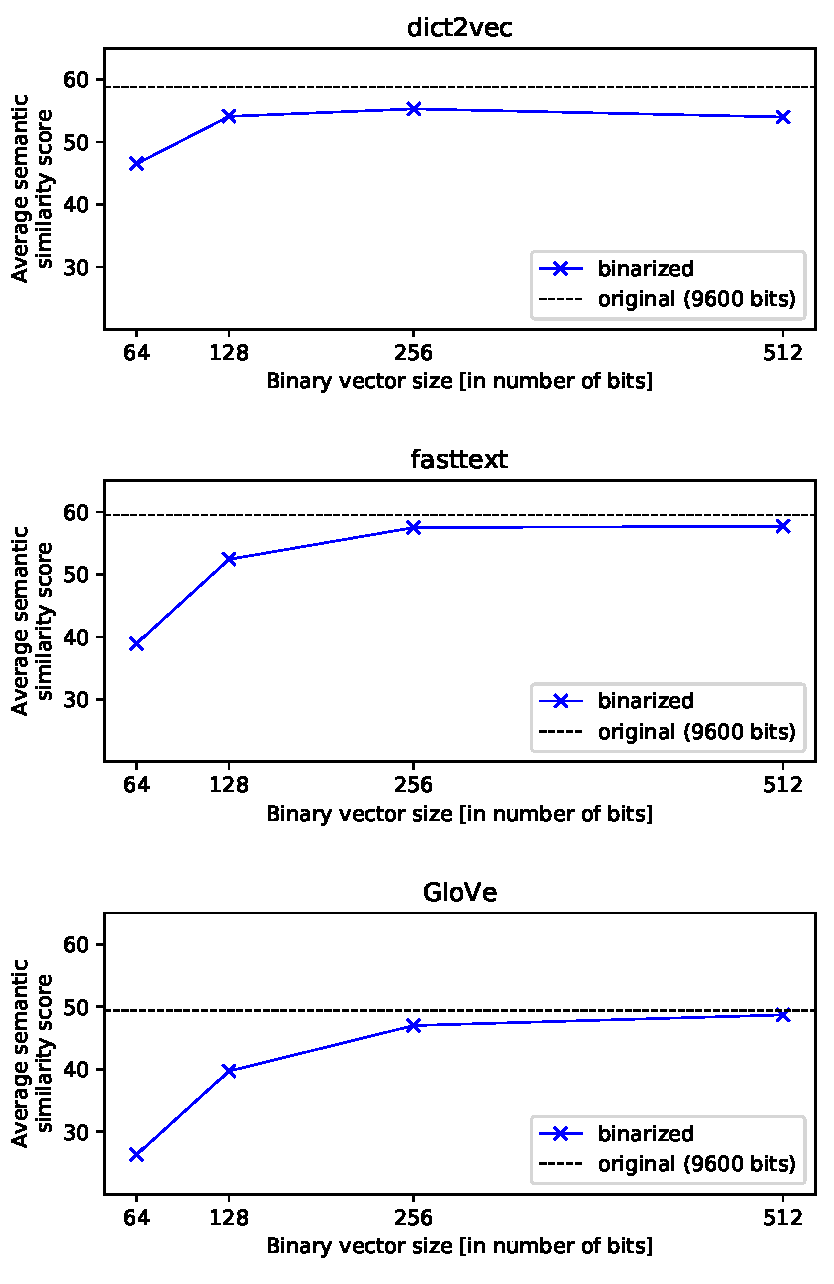
\includegraphics[width=0.75\linewidth]{ch06-binary-scores-plots}
        \caption[Scores of binary vectors on a word semantic similarity task.]
        {Average of the semantic similarity scores of all the datasets (computed
        with Fisher's transformation) for binary vectors of different sizes on a
        word semantic similarity task with different kinds of pre-trained
        vectors. The \textit{original} baseline indicates the average scores
        obtained with the pre-trained real-valued embeddings.}
        \label{ch06:img:plot-binary-vectors}
      \end{figure}

    \subsubsection{Word analogy}
      \autoref{ch06:tab:results-binary-analogies} reports the scores of binary
      vectors on a word analogy task for semantic and syntactic analogies.
      Although the best scores are also obtained with larger binary codes (512
      bits) like in the word semantic similarity task, the scores of binary
      vectors are lower than for real-valued vectors. This can be explained by
      the fact that the word analogy task is not suited to evaluate binary
      vectors. With real-valued vectors, analogies are found with vector
      additions and subtractions in the $\mathbb{R}^d$ space. In the binary
      space (where each value is either 0 or 1), adding or subtracting vectors
      does not make sense (like subtracting the bit 1 from the bit 0), resulting
      in lower scores of binary vectors on this analogy task.

      % Table with scores of binary vectors on word analogy task.
      \begin{table}[h]
        \centering
        \resizebox{\linewidth}{!}{
          \begin{tabular}{@{}lcccccrcccccrccccc@{}}
          \toprule[0.15em]
            & \multicolumn{5}{c}{\texttt{dict2vec}} & \phantom{}
            & \multicolumn{5}{c}{\texttt{fasttext}} & \phantom{}
            & \multicolumn{5}{c}{\texttt{GloVe}}\\

            \cmidrule(lr){2-6} \cmidrule(lr){8-12} \cmidrule(lr){14-18}
            & $\mathbb{R}$ & 64 & 128 & 256 & 512 &
            & $\mathbb{R}$ & 64 & 128 & 256 & 512 &
            & $\mathbb{R}$ & 64 & 128 & 256 & 512 \\
            \midrule
              % raw  64     128         256       512
            Semantic & 59.6 &&&&&& 37.6 &&&&&& 77.4\\
              \multicolumn{1}{c}{\texttt{NLB}}
                &-& 2.6 & 12.0 & 26.7 & \textbf{30.1} &
                &-& 2.3 & 7.5  & 18.0 & \textbf{25.0} &
                &-& 8.5 & 26.7 & 53.4 & \textbf{65.3}\\
              \multicolumn{1}{c}{\texttt{LSH}}
                &-& 0.8 &  4.6 & 14.9 & 29.9 &
                &-& 0.8 &  6.4 & 13.0 & 20.4 &
                &-& 6.1 & 25.9 & 47.9 & 59.3\\\\

            Syntactic & 54.0 &&&&&& 87.4 &&&&&& 67.0\\
              \multicolumn{1}{c}{\texttt{NLB}}
                &-& 3.5 & 16.7 & 34.8 & \textbf{36.2} &
                &-& 8.0 & 34.5 & 57.3 & 64.7 &
                &-& 7.3 & 23.9 & 46.3 & \textbf{52.4}\\
              \multicolumn{1}{c}{\texttt{LSH}}
                &-& 1.7 &  7.8 & 23.4 & 35.8 &
                &-& 4.0 & 21.5 & 46.2 & \textbf{65.7} &
                &-& 5.6 & 21.6 & 39.1 & 52.3\\
          \bottomrule[0.15em]
        \end{tabular}}
        \caption[Evaluation of binary and real-valued vectors on a word analogy
        task.] {Percentage of correctly predicted word analogies on several
        datasets (semantic and syntactic analogies) for binary vectors produced
        with the proposed method (\texttt{NLB} row) or produced with the Local
        Sensitive Hashing method (\texttt{LSH} row) with different vector sizes:
        64, 128, 256 and 512 bits. Several pre-trained word embeddings have been
        binarized (\texttt{dict2vec}, \texttt{fasttext} and \texttt{GloVe}). For
        each dataset, scores of original real-valued vectors are also reported
        ($\mathbb{R}$ column).}
        \label{ch06:tab:results-binary-analogies}
      \end{table}

    \subsubsection{Text classification}
      \autoref{ch06:tab:results-binary-classification} reports the accuracy
      scores obtained on different datasets in the text classification tasks for
      binary vectors learned by the \texttt{NLB} autoencoder model (\texttt{NLB}
      row) and original real-valued vectors ($\mathbb{R}$ column). In all the
      text classification tasks, binary vectors achieve their best scores with
      512 bits in general. Like for the word semantic similarity task, binary
      vectors are sometimes better than real-valued vectors. This is especially
      true for the 512-bit \texttt{fasttext} binarized vectors where the
      accuracy goes from $95.0$ to $97.3$ on DBpedia or from $49.0$ to $49.8$ on
      Amazon Full reviews. Using binarized vectors of less than 512 bits leads
      to better compression rates (because fewer bits are needed to encode each
      vector) but it causes a slight decrease in performances. The 256-bit
      binary vectors of \texttt{GloVe} are 37.5 times smaller than the original
      real-valued word embeddings (whose size is 9,600 bits per vector) but the
      accuracy drops between $0.4\%$ and $2.5\%$ depending on the dataset. The
      64-bit binary vectors of \texttt{dict2vec} (compression rate of 150) have
      a loss of accuracy of about $4\%$ on AG-News and DBpedia, about $11\%$ on
      Yahoo Answers and about $16\%$ on Amazon Full reviews compared to the
      scores obtained by real-valued vectors. The two latter datasets (Yahoo
      Answers and Amazon Full reviews) are the biggest ones, with respectively
      1.4M and 3M training samples while AG-News and DBpedia respectively
      contain 120k and 560k training samples. As the dataset becomes larger, the
      amount of information required to correctly classify documents also
      increases, so is the accuracy loss on those datasets when small binary
      vectors are used. Overall, these experiments show once again that binary
      embeddings are competitive with real-valued ones.

      % Table with scores of binary vectors on text classification tasks
      \begin{table}[h]
        \centering
        \resizebox{\linewidth}{!}{
          \begin{tabular}{@{}lcccccrcccccrccccc@{}}
          \toprule[0.15em]
            & \multicolumn{5}{c}{\texttt{dict2vec}} & \phantom{}
            & \multicolumn{5}{c}{\texttt{fasttext}} & \phantom{}
            & \multicolumn{5}{c}{\texttt{GloVe}}\\

            \cmidrule(lr){2-6} \cmidrule(lr){8-12} \cmidrule(lr){14-18}
            & $\mathbb{R}$ & 64 & 128 & 256 & 512 &
            & $\mathbb{R}$ & 64 & 128 & 256 & 512 &
            & $\mathbb{R}$ & 64 & 128 & 256 & 512 \\
            \midrule
              % raw  64     128         256       512
            AG-News & 89.0 &&&&&& 86.9 &&&&&& 89.5\\
              \multicolumn{1}{c}{\texttt{NLB}}
                &-& 85.3 & 85.9 & 87.7 & 87.8 &
                &-& 84.5 & 85.9 & 87.3 & 87.7 &
                &-& 84.0 & 87.2 & 88.5 & 88.5\\
              \multicolumn{1}{c}{\texttt{LSH}}
                &-& 78.8 & 82.6 & 86.1 & \textbf{88.1} &
                &-& 77.5 & 83.3 & 86.1 & \textbf{88.8} &
                &-& 83.5 & 86.6 & 88.4 & \textbf{88.6}\\\\

            DBpedia & 97.6 &&&&&& 95.0 &&&&&& 97.2\\
              \multicolumn{1}{c}{\texttt{NLB}}
                &-& 94.1 & 96.1 & 97.0 & 97.3 &
                &-& 91.7 & 95.1 & 96.6 & \textbf{97.3} &
                &-& 90.9 & 95.0 & 96.8 & \textbf{97.2}\\
              \multicolumn{1}{c}{\texttt{LSH}}
                &-& 89.6 & 94.2 & 96.5 & \textbf{97.4} &
                &-& 87.4 & 93.8 & 96.2 & 97.2 &
                &-& 90.4 & 94.2 & 96.3 & 97.2\\

            \midrule
            Yahoo Ans. & 68.1 &&&&&& 67.2 &&&&&& 68.1\\
              \multicolumn{1}{c}{\texttt{NLB}}
                &-& 60.7 & 63.8 & 66.0 & 66.8 &
                &-& 60.4 & 63.9 & 66.4 & \textbf{67.8} &
                &-& 57.5 & 62.5 & 66.4 & 66.1\\
              \multicolumn{1}{c}{\texttt{LSH}}
                &-& 52.3 & 59.9 & 64.5 & \textbf{67.1} &
                &-& 52.2 & 59.5 & 64.9 & 66.9 &
                &-& 56.8 & 62.0 & 65.3 & \textbf{67.0}\\
            \midrule

            Amazon Full & 47.5 &&&&&& 49.0 &&&&&& 47.1\\
              \multicolumn{1}{c}{\texttt{NLB}}
                &-& 39.9 & 43.9 & 46.8 & 47.7 &
                &-& 39.0 & 43.9 & 47.9 & \textbf{49.8} &
                &-& 37.4 & 42.6 & 46.7 & 47.8\\
              \multicolumn{1}{c}{\texttt{LSH}}
                &-& 38.3 & 42.5 & 45.6 & \textbf{48.1} &
                &-& 38.6 & 42.7 & 47.3 & 49.5 &
                &-& 37.9 & 43.0 & 45.9 & \textbf{48.6}\\\\

            Amazon Pol. & 84.2 &&&&&& 85.6 &&&&&& 83.8\\
              \multicolumn{1}{c}{\texttt{NLB}}
                &-& 76.3 & 80.7 & 83.2 & 83.8 &
                &-& 75.1 & 80.2 & 84.5 & \textbf{85.8} &
                &-& 73.1 & 78.9 & 83.2 & 84.4\\
              \multicolumn{1}{c}{\texttt{LSH}}
                &-& 74.3 & 79.0 & 81.9 & \textbf{84.5} &
                &-& 73.8 & 78.5 & 83.4 & 85.7 &
                &-& 74.7 & 79.1 & 82.1 & \textbf{85.0}\\\\

            Yelp Full & 52.5 &&&&&& 52.1 &&&&&& 52.7\\
              \multicolumn{1}{c}{\texttt{NLB}}
                &-& 45.1 & 48.7 & 51.6 & 52.0 &
                &-& 44.2 & 49.7 & 53.0 & \textbf{54.6} &
                &-& 42.7 & 48.4 & 51.8 & 53.2\\
              \multicolumn{1}{c}{\texttt{LSH}}
                &-& 43.0 & 47.7 & 51.0 & \textbf{53.1} &
                &-& 44.3 & 47.6 & 52.4 & 54.3 &
                &-& 43.6 & 48.2 & 51.5 & \textbf{53.4}\\\\
            Yelp Pol. & 87.8 &&&&&& 88.0 &&&&&& 87.9\\
              \multicolumn{1}{c}{\texttt{NLB}}
                &-& 80.8 & 84.5 & 86.6 & 87.6 &
                &-& 80.1 & 84.5 & 88.1 & 89.5 &
                &-& 77.8 & 84.2 & 86.9 & \textbf{88.7}\\
              \multicolumn{1}{c}{\texttt{LSH}}
                &-& 77.9 & 82.8 & 86.1 & \textbf{88.0} &
                &-& 80.3 & 82.2 & 87.2 & \textbf{89.8} &
                &-& 79.0 & 83.1 & 86.6 & 88.6\\
          \bottomrule[0.15em]
        \end{tabular}}
        \caption[Evaluation of binary and real-valued vectors on text
        classification tasks.] {Accuracy of correctly predicted labels in
        document classification (top), question classification (middle) and
        sentiment analysis (bottom) on several datasets for binary vectors
        produced with the proposed method (\texttt{NLB} row) or produced with
        the Local Sensitive Hashing methods (\texttt{LSH} row) with different
        vector sizes: 64, 128, 256 and 512 bits. For each dataset, scores of
        original real-valued vectors are also reported ($\mathbb{R}$ column).}
        \label{ch06:tab:results-binary-classification}
      \end{table}

  \subsection{Reconstructed word embeddings performances}
    \label{ch06:subsec:performances-reconstructed}
    \subsubsection{Word semantic similarity and word analogy}
      \label{ch06:subsubsec:results-reconstructed-intrinsic}
      \autoref{ch06:tab:results-reconstructed-semantic-analogies} reports the
      scores obtained on a word semantic similarity and on a word analogy tasks
      using the reconstructed real-valued vectors (\textit{recons.} row).
      Reconstructed vectors are computed with the decoder part of the
      \texttt{NLB} autoencoder and the learned latent binary vectors of the
      model, which explains why there are as many different reconstructed
      vectors as there are different sizes of binary vectors. \medskip

      For the word semantic similarity task (results in the top part
      in~\autoref{ch06:tab:results-reconstructed-semantic-analogies}),
      \texttt{fasttext} and \texttt{dict2vec} work best in most cases using
      256-bit binary vectors while \texttt{GloVe} requires larger binary vectors
      (512 bits) to reconstruct good real-valued vectors. On most datasets,
      vectors reconstructed from the 512-bit \texttt{GloVe} binary vectors
      outperforms the original real-valued vectors: $0.382$ against $0.371$ on
      SimLex, $0.247$ against $0.227$ on SimVerb and $0.620$ against $0.609$ on
      WordSim. For \texttt{dict2vec} and \texttt{fasttext}, binarizing and then
      reconstructing real-valued vectors from the binary vectors causes a loss
      of performances compared to the scores of original word vectors: between
      $-4.8\%$ (on WordSim) and $-11.7\%$ (on RW) for \texttt{dict2vec}; between
      $-8.2\%$ (on WordSim) and $-28.1\%$ (on SimVerb) for \texttt{fasttext}.
      The performance loss of reconstructed vectors is larger for
      \texttt{fasttext} than for \texttt{dict2vec} due to their different word
      embedding learning method. \texttt{fasttext} also encodes additional
      morphological information into word vectors by considering that a word is
      the sum of its subwords, which is harder to reconstruct after a dimension
      reduction (the binarization). \bigskip % so next paragraph is on next page

      \noindent For the word analogy task (results in the bottom part
      in~\autoref{ch06:tab:results-reconstructed-semantic-analogies}), scores of
      reconstructed vectors are far from the original ones: $-39\%$ for
      \texttt{dict2vec}, $-49\%$ for \texttt{fasttext} and $-19\%$ for
      \texttt{GloVe} (average loss of semantic and syntactic scores).
      \texttt{GloVe} reconstructed vectors have a smaller loss of performances
      compared to \texttt{dict2vec} and \texttt{fasttext}: since the number of
      vectors to binarize is smaller for \texttt{GloVe} embeddings, the model
      can preserve the arithmetic relations between vectors more easily. The low
      performances of reconstructed vectors is also a consequence of the low
      performances of binary vectors on this task: if analogy relations have not
      been preserved in the binary vector space during the binarization, then
      the model cannot recreate them from the binary word vectors.

      % Table with scores of reconstructed vectors on intrinsic tasks.
      \begin{table}[h]
        \centering
        \resizebox{\linewidth}{!}{
          \begin{tabular}{@{}lcccccrcccccrccccc@{}}
          \toprule[0.15em]
            & \multicolumn{5}{c}{\texttt{dict2vec}} & \phantom{}
            & \multicolumn{5}{c}{\texttt{fasttext}} & \phantom{}
            & \multicolumn{5}{c}{\texttt{GloVe}}\\

            \cmidrule(lr){2-6} \cmidrule(lr){8-12} \cmidrule(lr){14-18}
            & $\mathbb{R}$ & 64 & 128 & 256 & 512 &
            & $\mathbb{R}$ & 64 & 128 & 256 & 512 &
            & $\mathbb{R}$ & 64 & 128 & 256 & 512 \\
            \midrule
              % raw  64     128         256       512
            MEN & 0.746 &&&&&& 0.807 &&&&&& 0.737\\
              \multicolumn{1}{c}{\textit{recons.}}
                &-& 0.645 & \textbf{0.696} & 0.678 & 0.647 &
                &-& 0.458 & 0.562 & \textbf{0.623} & 0.593 &
                &-& 0.436 & 0.505 & 0.685 & \textbf{0.722}\\\\

            RW & 0.505 &&&&&& 0.538 &&&&&& 0.412\\
              \multicolumn{1}{c}{\textit{recons.}}
                &-& 0.357 & 0.416 & \textbf{0.446} & 0.393 &
                &-& 0.289 & 0.316 & \textbf{0.457} & 0.441 &
                &-& 0.248 & 0.292 & 0.364 & \textbf{0.405}\\\\

            SimLex & 0.452 &&&&&& 0.441 &&&&&& 0.371\\
              \multicolumn{1}{c}{\textit{recons.}}
                &-& 0.304 & 0.379 & \textbf{0.424} & 0.393 &
                &-& 0.192 & 0.300 & \textbf{0.405} & 0.340 &
                &-& 0.196 & 0.191 & 0.342 & \textbf{0.382}\\\\

            SimVerb & 0.417 &&&&&& 0.356 &&&&&& 0.227\\
              \multicolumn{1}{c}{\textit{recons.}}
                &-& 0.237 & 0.354 & \textbf{0.375} & 0.294 &
                &-& 0.128 & 0.182 & \textbf{0.256} & 0.253 &
                &-& 0.080 & 0.124 & 0.221 & \textbf{0.247}\\\\

            WordSim & 0.725 &&&&&& 0.697 &&&&&& 0.609\\
              \multicolumn{1}{c}{\textit{recons.}}
                &-& 0.614 & \textbf{0.690} & 0.674 & 0.588 &
                &-& 0.365 & 0.536 & \textbf{0.640} & 0.536 &
                &-& 0.265 & 0.422 & 0.565 & \textbf{0.620}\\
            \midrule
            Semantic & 59.6 &&&&&& 37.6 &&&&&& 77.4\\
              \multicolumn{1}{c}{\textit{recons.}}
                &-& 2.6 & 10.2 & 22.8 & \textbf{30.9} &
                &-& 1.8 &  5.0 & 14.6 & \textbf{15.2} &
                &-& 7.7 & 23.0 & 49.1 & \textbf{62.8}\\\\

            Syntactic & 54.0 &&&&&& 87.4 &&&&&& 67.0\\
              \multicolumn{1}{c}{\textit{recons.}}
                &-& 3.6 & 16.1 & 31.2 & \textbf{37.5} &
                &-& 4.6 & 14.6 & 50.8 & \textbf{53.1} &
                &-& 7.3 & 21.7 & 44.6 & \textbf{54.0}\\
          \bottomrule[0.15em]
        \end{tabular}}
        \caption[Evaluation of vectors reconstructed from binary codes on
        intrinsic tasks.]{Scores of real-valued vectors reconstructed by the
        \texttt{NLB} autoencoder model (\textit{recons.} row) from learned
        binary vectors (of 64, 128, 256 and 512 bits) on a word semantic
        similarity task (top) and a word analogy task (bottom) for several
        datasets. For each dataset, scores of original real-valued vectors are
        also reported ($\mathbb{R}$ column).}
        \label{ch06:tab:results-reconstructed-semantic-analogies}
      \end{table}

    \subsubsection{Text classification}
      \autoref{ch06:tab:results-reconstructed-classification} reports the
      accuracy scores obtained on several extrinsic evaluation tasks (document
      classification, question classification and sentiment analysis) using the
      reconstructed real-valued vectors (\textit{recons.} row). As explained at
      the beginning of~\autoref{ch06:subsubsec:results-reconstructed-intrinsic},
      reconstructed vectors are computed with the decoder part of the
      \texttt{NLB} autoencoder and the learned latent binary vectors of the
      model. On downstream NLP tasks like document classification or sentiment
      analysis, the results of reconstructed vectors are very consistent: they
      exhibit close performances to binary word vectors, which in turn exhibit
      almost equal performances to the original vectors, independently of the
      initial pre-trained vectors used (\textit{e.g.} $51.6$ against $52.5$ for
      the 256-bit binary vectors of \texttt{dict2vec} on Yelp Full; $96.4$
      against $95.0$ for the 256-bit binary vectors of \texttt{fasttext} on
      DBpedia; $47.3$ against $47.1$ for the 512-bit binary vectors of
      \texttt{GloVe} on Amazon Full). Although the pairwise word semantic
      similarities are not perfectly preserved in the reconstructed vectors,
      text classification tasks only need vectors close enough for those of the
      same category but not necessarily very accurate within a category. This
      makes binary or reconstructed vectors good for real use case
      downstream tasks. The optimal number of bits required to reconstruct
      real-valued vectors with good performances in text classification tasks is
      the same as for the word semantic similarity task (256 bits for
      \texttt{dict2vec} and \texttt{fasttext}, 512 bits for \texttt{GloVe}).

      % Table with scores of reconstructed vectors on extrinsic tasks.
      \begin{table}[h]
        \centering
        \resizebox{\linewidth}{!}{
          \begin{tabular}{@{}lcccccrcccccrccccc@{}}
          \toprule[0.15em]
            & \multicolumn{5}{c}{\texttt{dict2vec}} & \phantom{}
            & \multicolumn{5}{c}{\texttt{fasttext}} & \phantom{}
            & \multicolumn{5}{c}{\texttt{GloVe}}\\

            \cmidrule(lr){2-6} \cmidrule(lr){8-12} \cmidrule(lr){14-18}
            & $\mathbb{R}$ & 64 & 128 & 256 & 512 &
            & $\mathbb{R}$ & 64 & 128 & 256 & 512 &
            & $\mathbb{R}$ & 64 & 128 & 256 & 512 \\
            \midrule
              % raw  64     128         256       512
            AG-News & 89.0 &&&&&& 86.9 &&&&&& 89.5\\
              \multicolumn{1}{c}{\textit{recons.}}
                &-& 85.2 & 86.3 & \textbf{87.9} & 87.2 &
                &-& 82.8 & 84.3 & \textbf{87.7} & 87.3 &
                &-& 83.9 & 87.7 & 88.6 & \textbf{89.2}\\\\

            DBpedia & 97.6 &&&&&& 95.0 &&&&&& 97.2\\
              \multicolumn{1}{c}{\textit{recons.}}
                &-& 94.0 & 95.9 & \textbf{96.8} & 96.6 &
                &-& 89.5 & 92.6 & \textbf{96.4} & 96.0 &
                &-& 91.2 & 95.2 & 96.8 & \textbf{97.0}\\
            \midrule
            Yahoo Ans. & 68.1 &&&&&& 67.2 &&&&&& 68.1\\
              \multicolumn{1}{c}{\textit{recons.}}
                &-& 60.8 & 63.8 & 65.9 & \textbf{66.0} &
                &-& 60.0 & 62.9 & 66.3 & \textbf{66.8} &
                &-& 58.4 & 64.3 & 66.7 & \textbf{67.0}\\
            \midrule
            Amazon Full & 47.5 &&&&&& 49.0 &&&&&& 47.1\\
              \multicolumn{1}{c}{\textit{recons.}}
                &-& 40.1 & 44.0 & \textbf{46.8} & 46.2 &
                &-& 39.1 & 43.8 & 48.1 & \textbf{48.5} &
                &-& 39.8 & 45.3 & 47.1 & \textbf{47.3}\\\\

            Amazon Pol. & 84.2 &&&&&& 85.6 &&&&&& 83.8\\
              \multicolumn{1}{c}{\textit{recons.}}
                &-& 76.6 & 80.8 & \textbf{83.2} & 82.4 &
                &-& 75.1 & 80.2 & 84.7 & \textbf{84.8} &
                &-& 76.6 & 80.2 & 83.6 & \textbf{83.7}\\\\

            Yelp Full & 52.5 &&&&&& 52.1 &&&&&& 52.7\\
              \multicolumn{1}{c}{\textit{recons.}}
                &-& 45.3 & 48.8 & \textbf{51.6} & 50.9 &
                &-& 43.5 & 47.8 & 53.0 & \textbf{53.1} &
                &-& 43.4 & 50.3 & 52.3 & \textbf{52.8}\\\\

            Yelp Pol. & 87.8 &&&&&& 88.0 &&&&&& 87.9\\
              \multicolumn{1}{c}{\textit{recons.}}
                &-& 80.9 & 84.5 & \textbf{86.6} & 86.1 &
                &-& 79.6 & 84.0 & 88.2 & \textbf{88.5} &
                &-& 78.6 & 85.7 & 87.5 & \textbf{87.7}\\
          \bottomrule[0.15em]
        \end{tabular}}
        \caption[Evaluation of vectors reconstructed from binary codes on
        classification tasks.]{Accuracy of correctly predicted labels in
        document classification (top), question classification (middle) and
        sentiment analysis (bottom) on several datasets for real-valued vectors
        reconstructed by the \texttt{NLB} autoencoder model (\textit{recons.}
        row) from learned binary vectors of 64, 128, 256 and 512 bits. For each
        dataset, scores of original real-valued vectors are also reported
        ($\mathbb{R}$ column).}
        \label{ch06:tab:results-reconstructed-classification}
      \end{table}

  \subsection{Speed improvements in top-K queries}
    \label{ch06:subsec:performances-speed}
    The execution time (in milliseconds) of top-K queries benchmarks for
    binarized and original real-valued \texttt{GloVe} vectors are reported
    in~\autoref{ch06:tab:results-topk}. The first three rows (Top 1, Top 10 and
    Top 50) indicate the time used by the program to perform the query
    \textit{after} the vectors are loaded into the memory \textit{i.e.} the time
    needed to linearly scan all the vectors, compute the similarity with the
    query vector and select the $K$ highest values. For binary vectors, the
    Sokal \& Michener similarity is used while real-valued vectors use the
    cosine similarity. Finding the 10 closest vectors of a query vector is
    \textbf{30 times faster} with 256-bit binarized \texttt{GloVe} vectors than
    with the real-valued vectors and it can be up to 36 times faster with 64-bit
    binary vectors. Having faster computations of vector similarities is not the
    only interest of binary vectors. Since they take less space in memory, they
    are also much faster to load. The last row
    in~\autoref{ch06:tab:results-topk} indicates the time needed to load the
    vectors from a file (stored on a SSD) into the memory (stored in RAM) and
    perform a top-10 query. It takes 23.5 seconds to load the real-valued
    vectors and run the query whereas it only takes 310 milliseconds to do it
    with 256-bit binary vectors, which is \textbf{75 times faster}.

    \begin{table}[h]
      \centering
      \begin{tabular}{cccccc}
        \toprule[0.15em]
        Top-K query      & 64-bit & 128-bit & 256-bit & 512-bit & Real-valued\\
        \midrule
        Top 1            &  2.71  &   2.87  &   3.23  &   4.28  &   97.89    \\
        Top 10           &  2.72  &   2.89  &   3.25  &   4.29  &   98.08    \\
        Top 50           &  2.75  &   2.91  &   3.27  &   4.32  &   98.44    \\
        Loading + Top 10 &  160   &   213   &   310   &   500   &   23500    \\
        \bottomrule[0.15em]
      \end{tabular}
      \caption[Execution time to run a top-K query on binary and real-valued
      vectors.]{Execution time (in milliseconds) to run a top-K query on binary
      and real-valued vectors. For the first three rows (Top 1, Top 10 and Top
      50), the time needed to read and load the vectors into the memory is not
      taken into account. The loading time of vectors from the disk into the
      memory is only counted in the last row.}
      \label{ch06:tab:results-topk}
    \end{table}

  \subsection{Comparison with the naive approach}
    \label{ch06:subsec:performances-naive}
    A naive approach to produce binary vectors from pre-trained word embeddings
    is to map negative values of vectors to 0 and positive values to 1.
    Unfortunately, binary vectors produced with this method have the same number
    of bits as the the number of dimensions of original real-valued vectors.
    Since most pre-trained word vectors are not available in 64, 128 or 256
    dimensions, binarized vectors are not aligned with CPU registers by using
    the naive binarization method, which is an important requirement to achieve
    fast vector operations (see \autoref{ch06:sec:introduction} for a detailed
    explanation about the motivations to have binary vectors aligned with CPU
    registers). To produce aligned vectors with the naive method, one has first
    to train real-valued embeddings with 64, 128 or 256 dimensions and then
    apply the naive binarization approach to all vector values. First, this
    process is slower than using the \texttt{NLB} autoencoder model. It requires
    8 hours while the \texttt{NLB} autoencoder only needs 13 minutes to produce
    256-bit binary vectors from pre-trained \texttt{dict2vec} vectors. Second,
    binary vectors produced with the naive binarization have worse results than
    those produced with the \texttt{NLB} autoencoder model. For
    \texttt{dict2vec}, the average word semantic similarity scores are $0.447$
    and $0.496$ for the naive 64-bit and 128-bit binary vectors while the 64-bit
    and 128-bit \texttt{NLB} binary vectors achieve respectively $0.465$ and
    $0.541$.

  \subsection{Comparison with other binarization methods}
    \label{ch06:subsec:performances-others}
    The \textit{Locality Sensitive Hashing} method (\texttt{LSH}) is used to
    produce binary vectors of 64, 128, 256 and 512 bits from the same
    real-valued vectors as the \texttt{NLB} autoencoder model. They are
    evaluated on the same tasks as the \texttt{NLB} method and their scores are
    reported in~\autoref{ch06:tab:results-binary-semantic} for the word semantic
    similarity task, in~\autoref{ch06:tab:results-binary-analogies} for the word
    analogy task and in~\autoref{ch06:tab:results-binary-classification} for the
    text classification tasks. On the word semantic similarity and the word
    analogy tasks, \texttt{NLB} binary vectors are always better than the
    \texttt{LSH} ones (\textit{e.g.} $0.703$ against $0.638$ for the 512-bit
    binary vectors of \texttt{fasttext} on WordSim; $34.8$ against $23.4$ for
    the 256-bit binary vectors of \texttt{dict2vec} on Syntactic analogies),
    except for the 64-bit binary vectors of \texttt{GloVe} and some 64-bit
    binary vectors of \texttt{fasttext}. On the classification tasks, 512-bit
    binary vectors of \texttt{NLB} are on par with the \texttt{LSH} ones, but
    the 128-bit and 256-bit binary vectors of \texttt{NLB} have better
    performances than the respective \texttt{LSH} vectors. The \texttt{NLB}
    model gives the best size to performance ratio for small binary vectors.
    \medskip

    \texttt{NLB} binary vectors have also been compared to the binary vectors
    produced by~\citep{faruqui2015sparse}.~\citeauthor{faruqui2015sparse} binary
    vectors are mostly sparse ($90\%$ of bits are set to the value $0$) and
    therefore are too large to be computationally interesting: the number of
    bits is set to $3,000$ in their method so they do not fit in CPU registers.
    They also have lower performances than the \texttt{NLB} binary vectors:
    $0.560$ for their average word semantic similarity score while the
    \texttt{NLB} model achieves $0.575$ with 256-bit binary vectors.

  \subsection{Qualitative analysis of binary embeddings}
    \label{ch06:subsec:qualitative-analysis}
    \subsubsection{Visualization of activated dimensions in binary vectors}
      In~\autoref{ch06:img:bits-visualization}, the 50 most similar (top) and
      the 50 least similar (bottom) vectors to the 512-bit vectors of 4 words
      (``queen'', ``automobile'', ``jupiter'' and ``man'') are plotted with red
      (resp. white) pixels for bits set to 1 (resp. 0). Some vertical stripes
      are clearly visible in top areas: similar binary vectors have common bits
      on many dimensions and therefore have the same pixel color for those
      dimensions. In bottom areas, no vertical patterns are visible because
      non-similar binary vectors do not have a lot of bits in common and
      therefore do not have the same pixel color on many dimensions. This
      visualization shows that binarized vectors have similar semantic
      properties as real-valued embeddings, which are known to encode common
      semantic features on common sets of dimensions.

      \begin{figure}[h]
        \centering
          % 0.94\textwidth is the max size the image can have before pushing the
          % next subssubsection on the next page and fucking up the formatting
          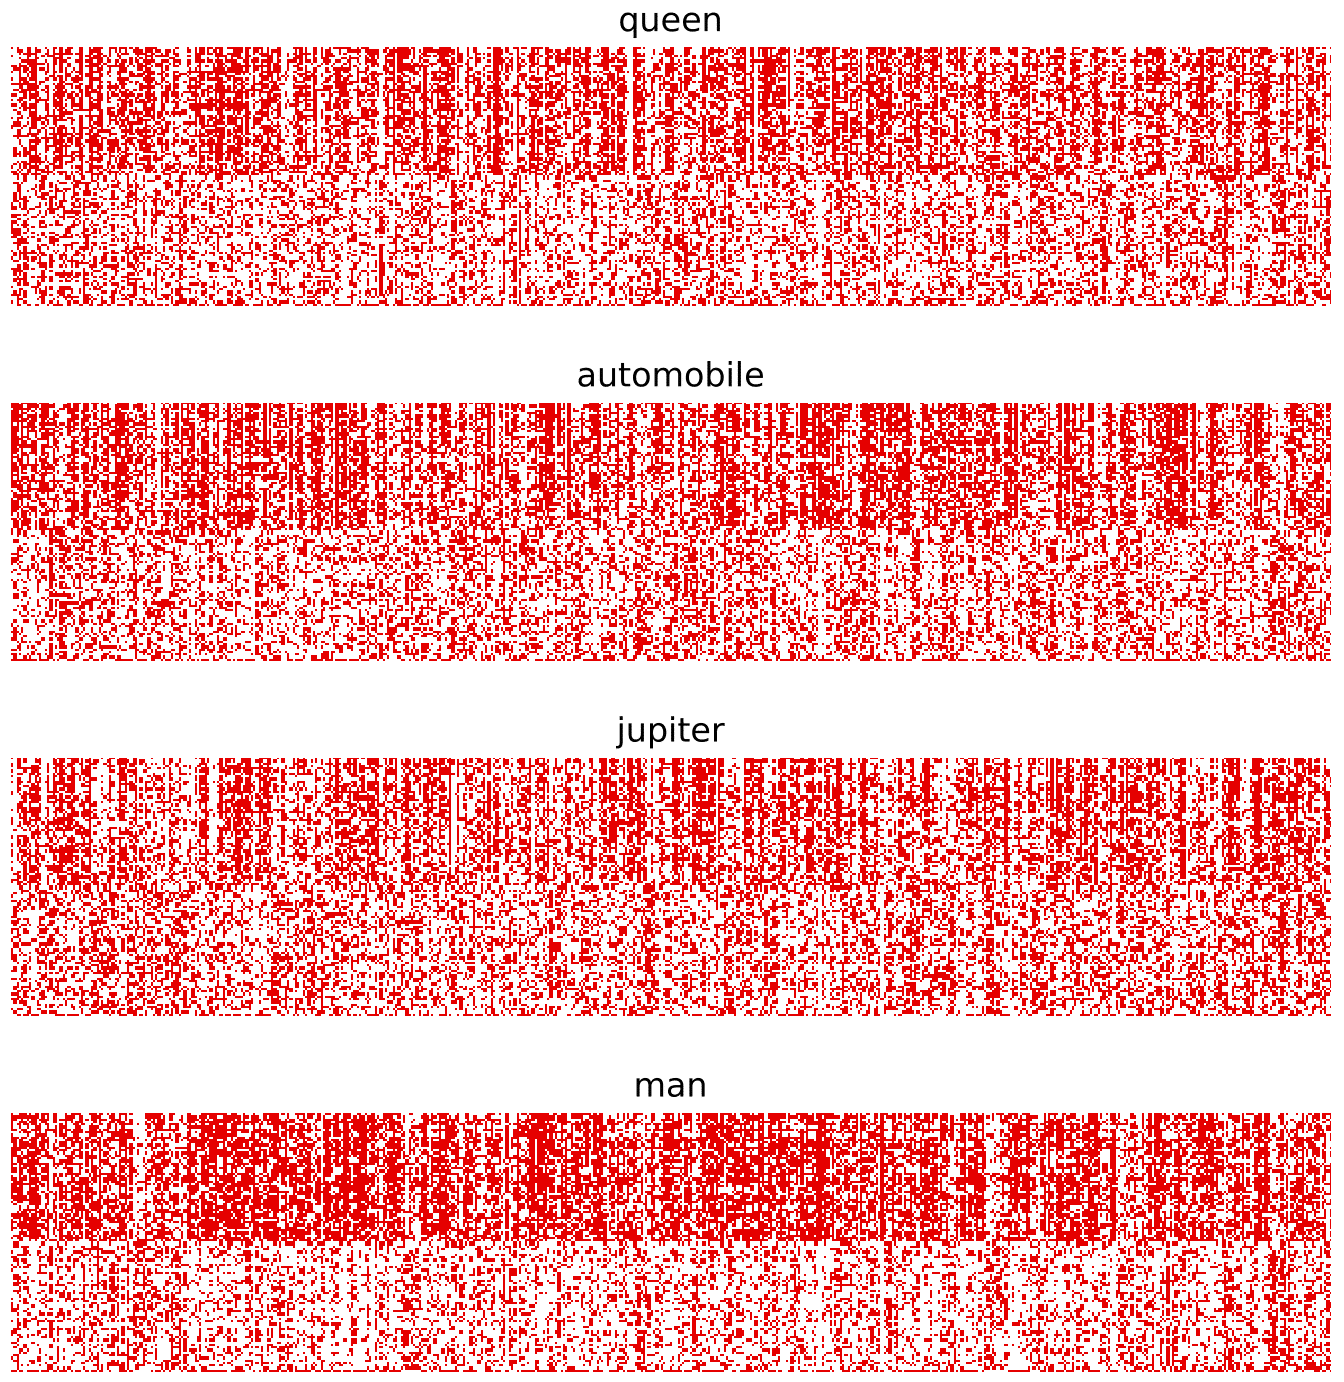
\includegraphics[width=0.94\textwidth]{ch06-activated-bits}
          \caption[Visualization of the activated bits in some binary
          vectors.]{Visualization of the activated bits (red pixels for 1,
          white pixels for 0) in the binary vectors of the 50 closest
          (top) and the 50 furthest (bottom) neighbors of vectors.}
          \label{ch06:img:bits-visualization}
      \end{figure}

    \subsubsection{Evolution of word vector similarity}
      The word semantic similarity task is based on datasets containing pairs of
      words associated to a value which represents the semantic similarity
      (evaluated by human annotators) between the words. For some pairs
      (reported in~\autoref{ch06:tab:evolution-semantic-similarity}), the
      similarity of the pre-trained real-valued vectors of the corresponding
      words is far from the human assigned value, but the similarity of the
      binarized version of the vectors is closer to the human assigned value,
      making the binary embeddings closer to the human semantic representation
      of words.
      % Table of evolution of similarity between pairs of words after binarized
      \begin{table}[h!]
        \centering
        \begin{tabular}{cccc}
          \toprule[0.15em]
          Words              & Human judgment & Binary similarity & Real-valued similarity   \\
          \midrule
          dollar -- buck     &    0.92        &  0.56             &  0.13 \\
          seafood -- sea     &    0.75        &  0.62             &  0.24 \\
          money -- salary    &    0.79        &  0.58             &  0.41 \\
          car -- automobile  &    0.98        &  0.69             &  0.60 \\
          \bottomrule[0.15em]
        \end{tabular}
        \caption[Evolution of semantic similarity of pairs of words after the
        binarization.]{Semantic similarity for some pairs of words, evaluated by
        human or computed with binary and real-valued vectors.}
        \label{ch06:tab:evolution-semantic-similarity}
      \end{table}

\section{Conclusion}
  Methods to learn word embeddings commonly associate a numerical vector to each
  word of a vocabulary. As the vocabulary gets bigger over the time because the
  size of training corpora is also largely increasing over the years, it is not
  uncommon to see word embeddings requiring several gigabytes in memory for
  storage. With new learning methods like contextual representations, the memory
  and computational power requirements are even bigger due to the huge number of
  parameters in the deep learning architectures involved. \medskip

  Although most of the word embeddings learning methods are trained on large
  computing servers without any problems, their important requirements of
  computing resources prevents their use on low-resource devices like
  smartphones because of their limited memory capacity and their small computing
  power. This shortcoming of such methods motivated the emergence of new
  approaches (presented in~\autoref{chap:methods-reduction}) to reduce the size
  of vector representations and to find new solutions to minimize the amount of
  computing power needed to perform vector operations, with methods such as
  vector quantization which takes advantage of CPU-optimized functions on
  integer or binary vectors to speed up vector computations. However, most of
  the existing methods to reduce the size of vectors or to accelerate vector
  computations are for fast similarity searches (\textit{i.e.} for vector
  retrieval tasks) not for using the size-reduced vectors in downstream NLP
  models. \medskip

  This chapter presented the second contribution of this thesis, to address the
  problem of finding word embeddings with small size in memory and which allow
  fast vector operations while preserving the linguistic properties of words so
  they can be used in downstream NLP models. It details a new autoencoder
  architecture with a binary latent representation to transform pre-trained
  real-valued word vectors into binary vectors of any size. This is particularly
  suitable when the size of binary vectors is the same as the CPU registers size
  because it allows a significant increase in vector operations computing speed.
  This method, named \texttt{NLB}, has the advantage of being simple yet
  powerful and allows to preserve the semantic information of the original
  pre-trained vectors into the binary word embeddings.\medskip

  Binary word embeddings produced with the \texttt{NLB} model exhibit almost the
  same performances as the original real-valued vectors on both word semantic
  similarity and text classification tasks. Furthermore, since the binary
  representations require less space in memory (a 256-bit binary vector is
  $97\%$ smaller than a traditional 300-dimensional real-valued word vector), it
  allows one to run a top-K query 30 times faster than with real-valued vectors
  since the binary similarity is much faster to compute than a regular cosine
  similarity. Additionally, it is possible to reconstruct real-valued vectors
  from the binary representations using the decoder part of the \texttt{NLB}
  autoencoder. Vectors reconstructed from the binary vectors exhibit similar
  performances on downstream tasks like document classification or sentiment
  analysis compared to the original pre-trained word vectors.

%% raw score of semantic similarity scores (Spearman)
%%
%%   dict2vec | naive | 64bits | 128bits | 256bits | 300bits | 512bits | real
%% ============================================================================
%%     MEN    | 0.679 |  0.661 |  0.713  |  0.703  |  0.686  |  0.713  | 0.746
%%     RW     | 0.455 |  0.365 |  0.420  |  0.456  |  0.456  |  0.456  | 0.505
%%  SimLex999 | 0.434 |  0.320 |  0.381  |  0.448  |  0.421  |  0.429  | 0.452
%%   SimVerb  | 0.366 |  0.253 |  0.366  |  0.384  |  0.371  |  0.355  | 0.417
%%    WS353   | 0.658 |  0.637 |  0.716  |  0.696  |  0.658  |  0.666  | 0.725
%% ---------------------------------------------------------------------------
%%    W.avg   | 0.497 |  0.421 |  0.497  |  0.513  |  0.500  |  0.503  | 0.550
%% Fisher.avg | 0.531 |  0.465 |  0.541  |  0.553  |  0.531  |  0.540  | 0.588
%%
%%
%%   fasttext | naive | 64bits | 128bits | 256bits | 300bits | 512bits | real
%% ============================================================================
%%     MEN    | 0.762 |  0.579 |  0.720  |  0.759  |  0.764  |  0.763  | 0.807
%%     RW     | 0.522 |  0.368 |  0.447  |  0.527  |  0.522  |  0.527  | 0.538
%%  SimLex999 | 0.434 |  0.251 |  0.380  |  0.446  |  0.443  |  0.430  | 0.441
%%   SimVerb  | 0.347 |  0.192 |  0.267  |  0.337  |  0.352  |  0.351  | 0.356
%%    WS353   | 0.720 |  0.503 |  0.691  |  0.700  |  0.696  |  0.703  | 0.697
%% ---------------------------------------------------------------------------
%%    W.avg   | 0.531 |  0.363 |  0.468  |  0.528  |  0.534  |  0.533  | 0.551
%% Fisher.avg | 0.580 |  0.389 |  0.524  |  0.575  |  0.577  |  0.577  | 0.595
%%
%%
%%    GloVe   | naive | 64bits | 128bits | 256bits | 300bits | 512bits | real
%% ============================================================================
%%     MEN    | 0.715 |  0.460 |  0.632  |  0.694  |  0.710  |  0.727  | 0.737
%%     RW     | 0.381 |  0.250 |  0.344  |  0.406  |  0.385  |  0.402  | 0.412
%%  SimLex999 | 0.393 |  0.204 |  0.313  |  0.372  |  0.388  |  0.367  | 0.371
%%   SimVerb  | 0.242 |  0.076 |  0.186  |  0.229  |  0.225  |  0.229  | 0.227
%%    WS353   | 0.603 |  0.299 |  0.448  |  0.563  |  0.580  |  0.602  | 0.609
%% ---------------------------------------------------------------------------
%%    W.avg   | 0.444 |  0.249 |  0.377  |  0.433  |  0.436  |  0.444  | 0.449
%% Fisher.avg | 0.486 |  0.263 |  0.397  |  0.470  |  0.477  |  0.487  | 0.494
